\section{转录组学概述}
\subsection{组学概述}
\begin{frame}
  \frametitle{转录组学 | 组学}
  \begin{figure}
    \centering
    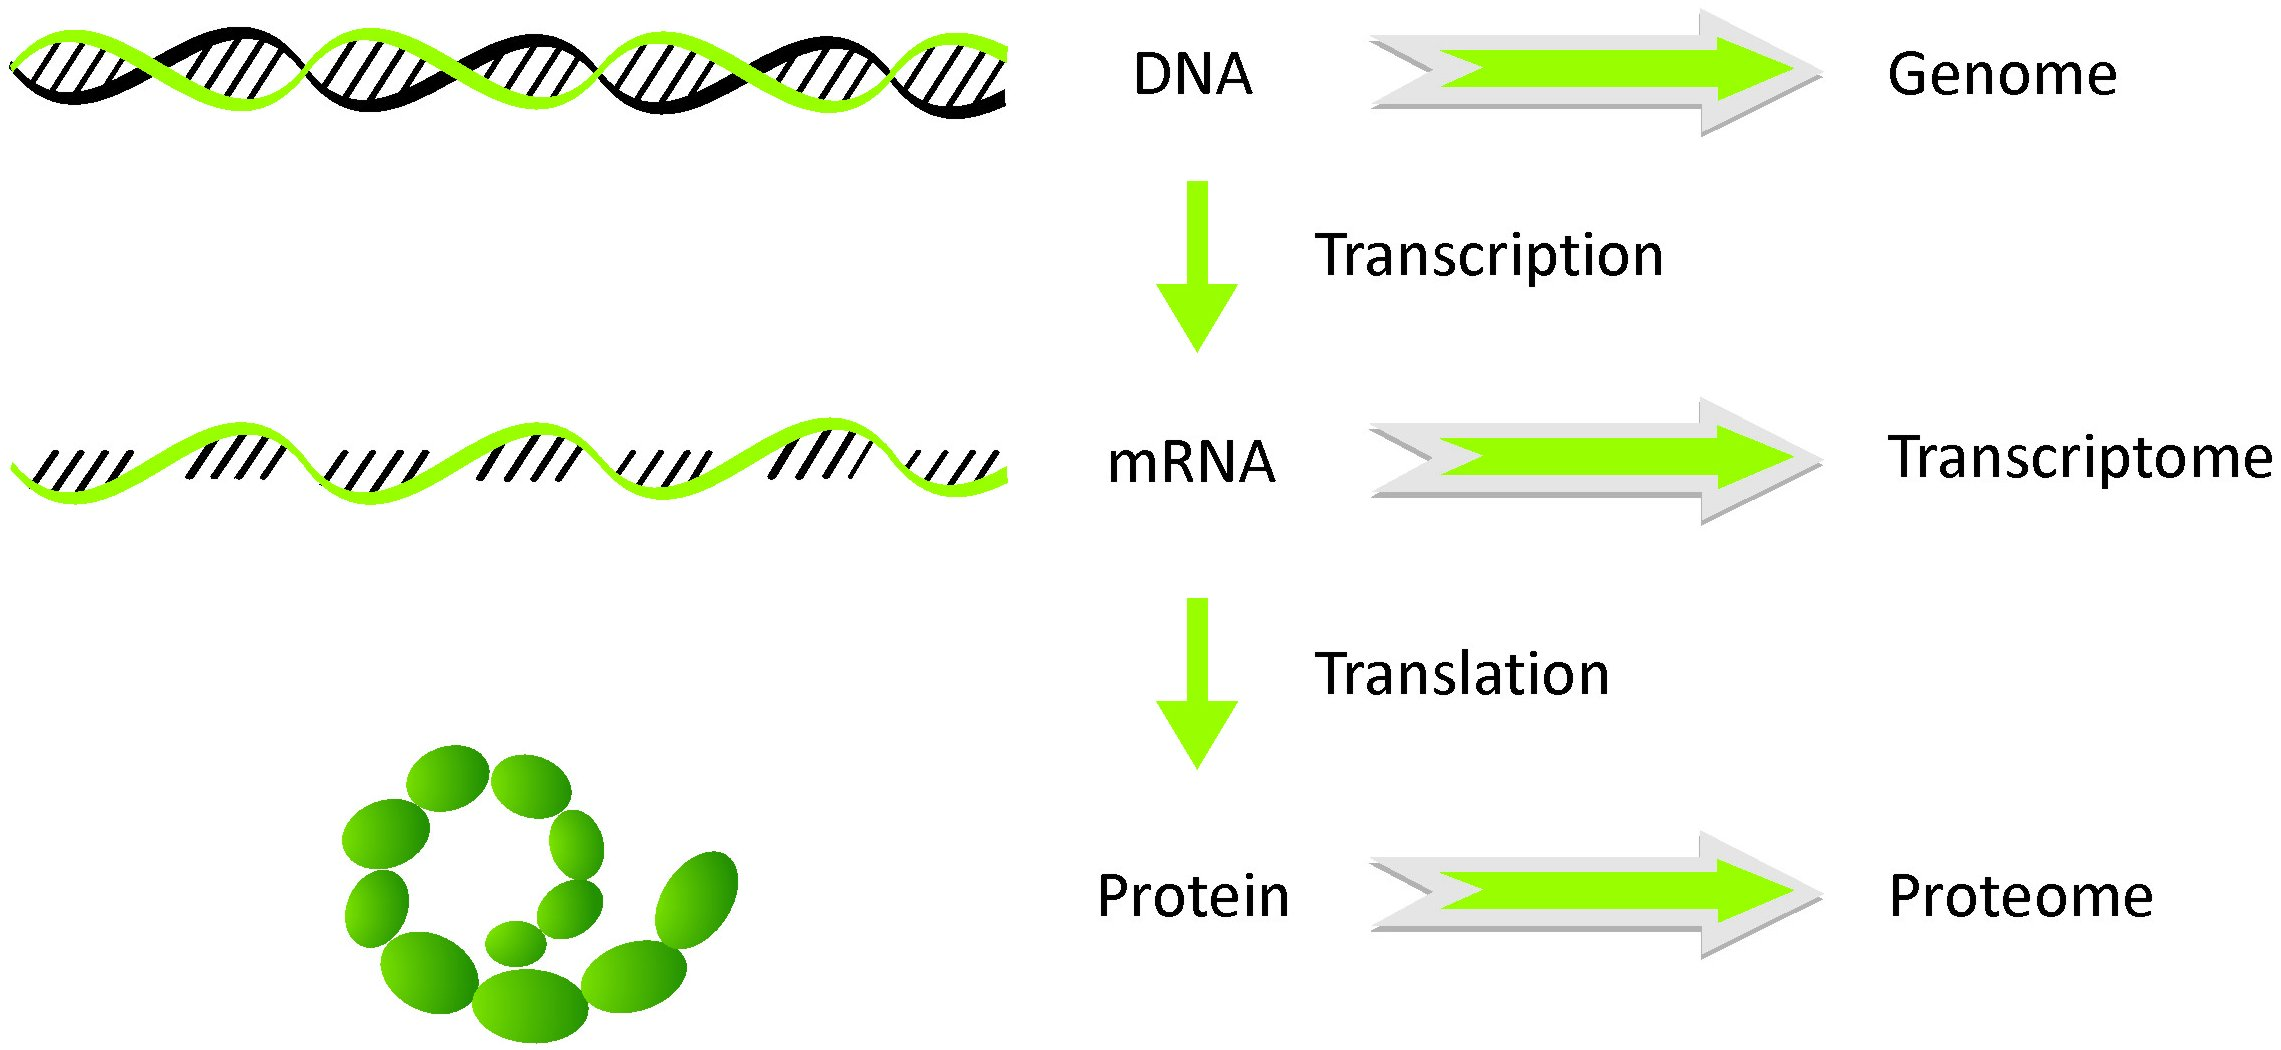
\includegraphics[width=0.9\textwidth]{c3_transcriptome/omics_01.jpg}
  \end{figure}
\end{frame}

\begin{frame}
  \frametitle{转录组学 | 组学}
  \begin{figure}
    \centering
    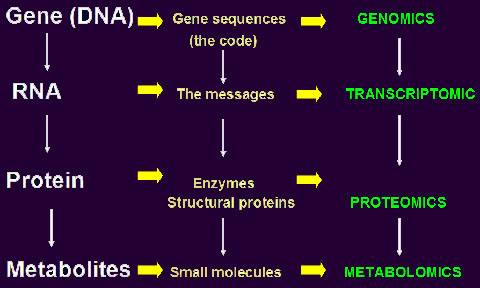
\includegraphics[width=0.9\textwidth]{c3_transcriptome/omics_02.jpg}
  \end{figure}
\end{frame}

\begin{frame}
  \frametitle{转录组学 | \textcolor{red}{组学}}
  \begin{figure}
    \centering
    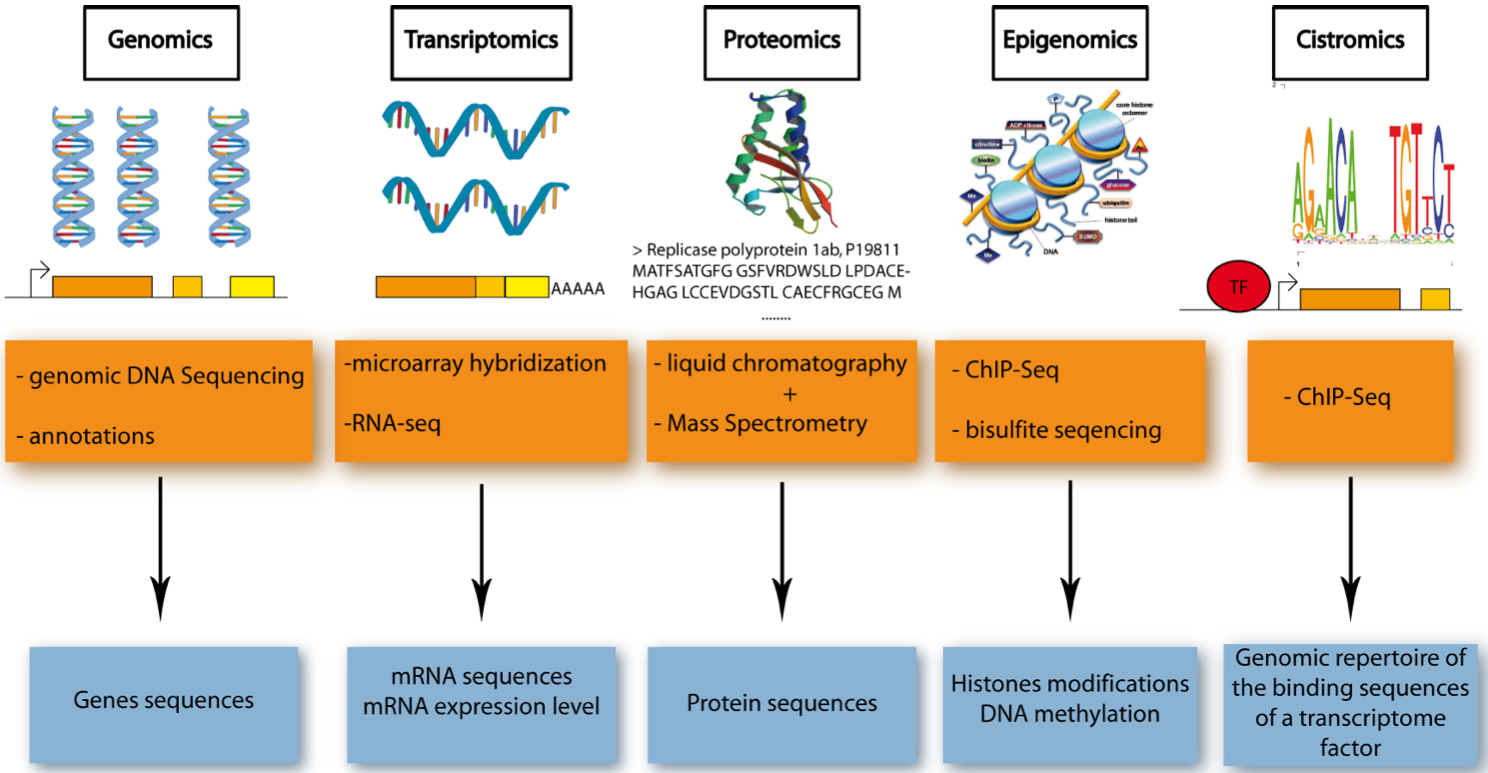
\includegraphics[width=0.95\textwidth]{c3_transcriptome/omics_03.png}
  \end{figure}
\end{frame}

\begin{frame}
  \frametitle{转录组学 | 组学}
  \begin{figure}
    \centering
    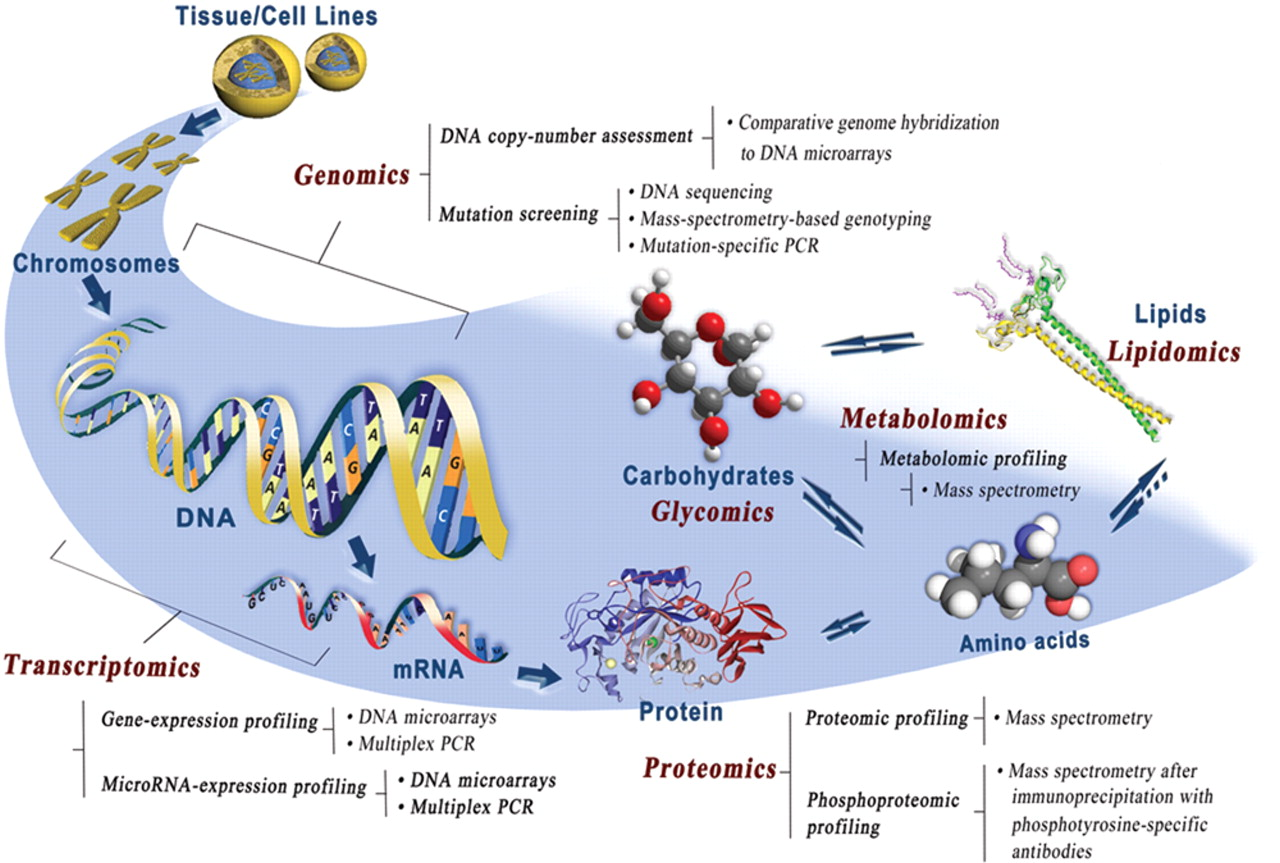
\includegraphics[width=0.9\textwidth]{c3_transcriptome/omics_04.jpg}
  \end{figure}
\end{frame}

\subsection{转录组学}
\begin{frame}
  \frametitle{转录组学 | 概述 | 基因表达}
  \begin{block}{基因表达}
 基因表达(gene expression)是用基因中的信息来合成基因产物的过程。产物通常是蛋白质,但对于非蛋白质编码基因,如转运RNA(tRNA)和小核RNA(snRNA),产物则是RNA。\\
 \vspace{0.5em}
基因表达的过程可分为转录、RNA剪接、翻译、蛋白质的翻译后修饰这几步。基因表达调控控制细胞的结构与功能,同时也是细胞分化、形态发生及生物体适应性的基础。不同的时间、不同的环境,以及不同部位的细胞,或是基因在细胞中的含量差异,皆可能使基因产生不同的表现。
  \end{block}
  \begin{figure}
    \centering
    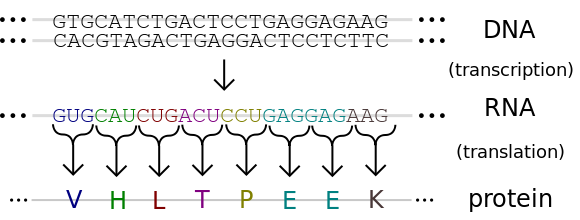
\includegraphics[width=0.7\textwidth]{c3_transcriptome/general_ge_01.png}
  \end{figure}
\end{frame}

\begin{frame}
  \frametitle{转录组学 | 概述 | 基因表达谱}
  \begin{block}{基因表达谱}
    基因表达谱(gene expression profile)是一种在分子生物学领域,借助cDNA、表达序列标签(EST)或寡核苷酸芯片来测定细胞基因表达情况(包括特定基因\textcolor{red}{是否表达}、\textcolor{red}{表达丰度}、不同组织、不同发育阶段以及不同生理状态下的\textcolor{red}{表达差异})的方法。\\
\vspace{1em}
通过一次性测定大量基因构建起细胞功能的总体态势图,可以从图谱中区分出正在分裂的细胞,以及细胞对于特征性治疗的反应。基因表达谱还有助于了解疾病的发病机制、药物的生理反应和治疗效果。\\
\vspace{1em}
基因表达图谱从逻辑上说是基因测序的下一个步骤:基因序列包含细胞可能存在的功能的信息,而基因表达谱则包含细胞实际上正在完成的工作的信息。
  \end{block}
\end{frame}

\begin{frame}
  \frametitle{转录组学 | 概述 | 基因表达谱}
  \begin{block}{Technique}
    \textcolor{red}{DNA microarray} technology measures the relative activity of \textcolor{red}{previously identified target genes}.\\
    \vspace{1em}
    Sequence based techniques, like serial analysis of gene expression (\textcolor{red}{SAGE, SuperSAGE}) are also used for gene expression profiling. SuperSAGE is especially accurate and can measure \textcolor{red}{any active gene}, not just a predefined set.\\
 \vspace{1em}
 The advent of next-generation sequencing has made sequence based expression analysis an increasingly popular, ``digital" alternative to microarrays called \textcolor{red}{RNA-Seq}. 
  \end{block}
\end{frame}

\begin{frame}
  \frametitle{转录组学 | 概述 | 转录组}
  \begin{block}{\textcolor{red}{转录组}}
转录组(transcriptome),也称为“转录物组”,广义上指在相同环境(或生理条件)下的在一个细胞、或一群细胞中所能转录出的所有RNA的总和,包括信使RNA(mRNA)、核糖体RNA(rRNA)、转运RNA(tRNA)及非编码RNA;狭义上则指细胞所能转录出的所有信使RNA(mRNA)。
  \end{block}
  \begin{figure}
    \centering
    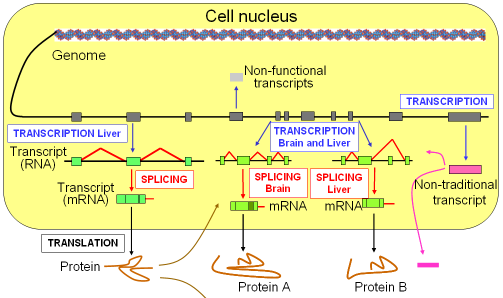
\includegraphics[width=0.65\textwidth]{c3_transcriptome/general_trans_01.png}
  \end{figure}
\end{frame}

\begin{frame}
  \frametitle{转录组学 | 概述 | 转录组}
  \begin{block}{转录组}
转录组这个术语可用于指代给定有机体中的转录本总集,或者是特定细胞类型中的特定转录本子集。\\
\vspace{0.5em}
不考虑突变,固定给定细胞株的基因组数量基本上是不变的;与之不同,转录物组可以随外部环境条件而有所变化。由于转录物组包括了所有在细胞里的mRNA的转录,除却异常的mRNA降解现象(例如转录衰减)以外,转录组反映了在任何给定时间内活跃表达的基因。\\
\vspace{0.5em}
转录物组学的研究,也被称为“基因表达谱”,检测了在一个特定的细胞群内的mRNA表达水平,通常采用基于DNA微阵列技术的高通量技术。使用新一代测序技术在核苷酸水平上来研究转录物组,被称为“RNA测序(RNA-Seq)”。
  \end{block}
\end{frame}

\begin{frame}
  \frametitle{转录组学 | 概述 | 转录组 | RNA-Seq}
  \begin{block}{Methods of construction}
    There are two general methods of inferring transcriptomes.
    \begin{itemize}
      \item One approach maps sequence reads onto a reference genome, either of the organism itself (whose transcriptome is being studied) or of a closely related species.
      \item The other approach, \textit{de novo} transcriptome assembly, uses software to infer transcripts directly from short sequence reads.
    \end{itemize}
  \end{block}
\end{frame}

\begin{frame}
  \frametitle{转录组学 | 概述 | 转录组学}
  \begin{block}{\textcolor{red}{转录组学}}
转录组学(或“转录物组学”,transcriptomics)是分子生物学的分支,负责研究在单个细胞或一个细胞群的特定细胞类型内所生产的mRNA分子。\\
    \vspace{0.5em}
转录组测定的是表达的基因数目。这个数目包括了在各种不同水平上表达的基因。\\
\end{block}
\end{frame}

\begin{frame}
  \frametitle{转录组学 | 概述 | 转录组学}
\begin{block}{丰度}
每个细胞里每一种mRNA分子的平均数称为该种mRNA的丰度。根据丰度可把mRNA群体分为两大类:
\begin{itemize}
  \item 高丰度mRNA组分。通常由每个细胞里不到100种的mRNA而每种mRNA分子由1000-10,000份备份所组成,通常占总mRNA的50\%左右。
  \item 除高丰度mRNA组分外,另一半mRNA由长约10,000nt的种类繁多的序列所组成,每种序列在mRNA中只有少量备份。称为“稀有mRNA”或“复杂mRNA”。
\end{itemize}
  \end{block}
\end{frame}

\begin{frame}
  \frametitle{转录组学 | 概述 | 转录组学}
  \begin{block}{转录组学}
大量表达的基因之间是有很大区别的。例如,卵清蛋白只在输卵管细胞里合成而不在肝脏内合成。它占输卵管内mRNA总量的一半。但是高丰度的mRNA只占表达基因数的很小一部分。根据生物体的基因数目以及不同类型细胞出现转录变化的基因数,人们需要了解不同表型细胞稀有mRNA基因相同的程度。\\
\vspace{1em}
稀有mRNA是普遍共有的。一个细胞中的mRNA序列只有10\%左右是该细胞独有的,大部分序列是许多(甚至是所有)类型的细胞所共有的。这提示哺乳动物中共有的基因数也许达10,000个,包括了各种类型细胞所需的功能。编码这种类型的功能的基因,有时被称为“\textcolor{red}{持家基因}”或“组成型基因”。这类功能不同于特定细胞表现型所需的特定功能(例如卵清蛋白或珠蛋白的功能)。编码特殊功能的基因称为“\textcolor{red}{奢侈基因}”。
  \end{block}
\end{frame}

\begin{frame}
  \frametitle{转录组学 | 概述 | 转录组学}
  \begin{block}{问题}
    \begin{itemize}
      \item 一个细胞、组织或生物体的全部RNA集合体中包括多少种RNA,各种RNA的数量有多少?
      \item 在不同发育时期和不同外界环境作用下RNA集合体会出现怎样的变化?
      \item 在细胞中转录是怎样被调节的?
      \item ……
    \end{itemize}
  \end{block}
  \pause
  \begin{block}{\textcolor{red}{转录组学}}
    转录组学(transcriptomics)是对转录水平上发生的事件及其相互关系和意义进行整体研究的一门学科。
  \end{block}
\end{frame}

\begin{frame}
  \frametitle{转录组学 | 概述 | 转录组学 | \textcolor{red}{研究内容}}
  \begin{block}{研究内容(4个水平)}
    \begin{itemize}
      \item 对特定细胞的转录与加工机制进行研究
      \item 对转录物编制目录便于进一步归类研究
      \item 绘制动态的转录物图形
      \item 转录物调控网络
    \end{itemize}
  \end{block}
\end{frame}

\begin{frame}
  \frametitle{转录组学 | 概述 | 转录组学 | 研究内容}
  \begin{figure}
    \centering
    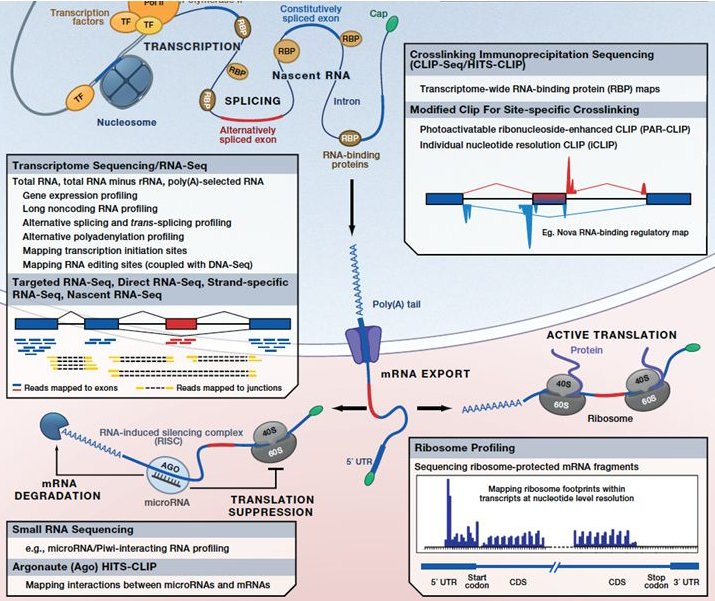
\includegraphics[width=0.75\textwidth]{c3_transcriptome/general_trans_content_01.jpg}
  \end{figure}
\end{frame}

\subsection{研究方法}
\begin{frame}
  \frametitle{转录组学 | 研究方法 | \textcolor{red}{概述}}
  \begin{figure}
    \centering
    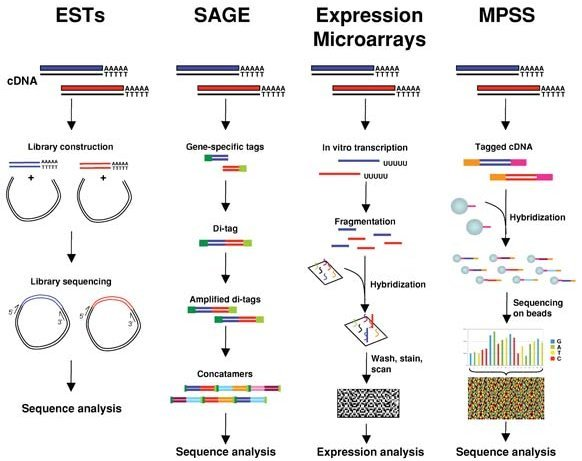
\includegraphics[width=0.8\textwidth]{c3_transcriptome/trans_method_01.jpg}
  \end{figure}
\end{frame}

\begin{frame}
  \frametitle{转录组学 | 研究方法 | \textcolor{red}{概述}}
  \begin{figure}
    \centering
    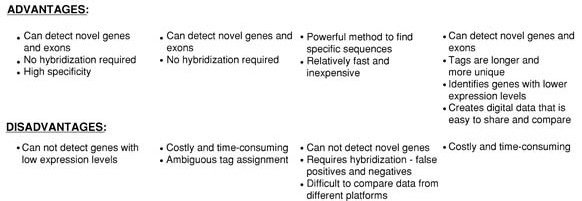
\includegraphics[width=0.9\textwidth]{c3_transcriptome/trans_method_02.jpg}
  \end{figure}
\end{frame}

\begin{frame}
  \frametitle{转录组学 | 研究方法 | 概述}
  \begin{figure}
    \centering
    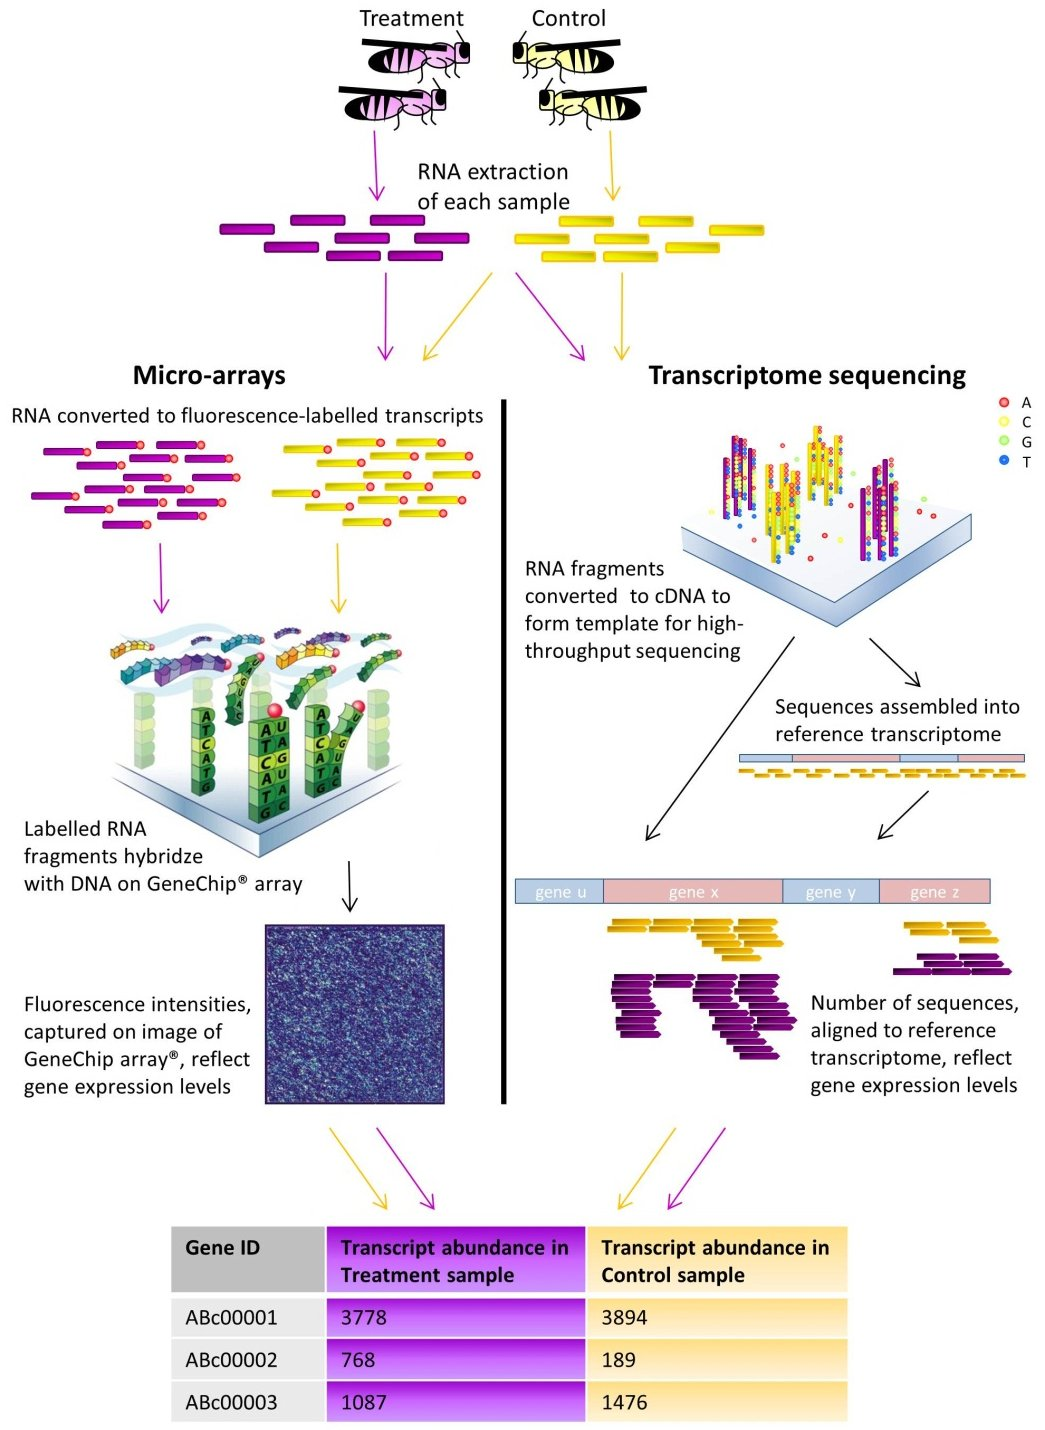
\includegraphics[width=0.5\textwidth]{c3_transcriptome/trans_method_03.jpg}
  \end{figure}
\end{frame}

\begin{frame}
  \frametitle{转录组学 | 研究方法 | EST}
  {\footnotesize
  \begin{block}{EST}
    EST(expressed sequence tag,表达序列标签)是从cDNA文库中生成的一些很短的序列(500~800bp),代表在特定组织或发育阶段表达的基因。\\
    \vspace{0.2em}
    In genetics, an expressed sequence tag or EST is a short sub-sequence of a cDNA sequence. ESTs may be used to identify gene transcripts, and are instrumental in gene discovery and in gene-sequence determination.
  \end{block}
  }
  \begin{figure}
    \centering
    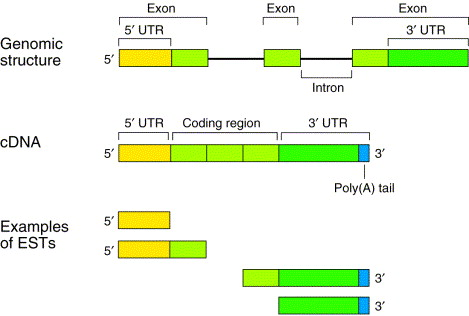
\includegraphics[width=0.6\textwidth]{c3_transcriptome/method_est_01.jpg}
  \end{figure}
\end{frame}

\begin{frame}
  \frametitle{转录组学 | 研究方法 | SAGE}
  \begin{block}{SAGE}
    Serial analysis of gene expression (SAGE) is a technique used by molecular biologists to produce a snapshot of the messenger RNA population in a sample of interest in the form of small tags that correspond to fragments of those transcripts.
  \end{block}
  \begin{figure}
    \centering
    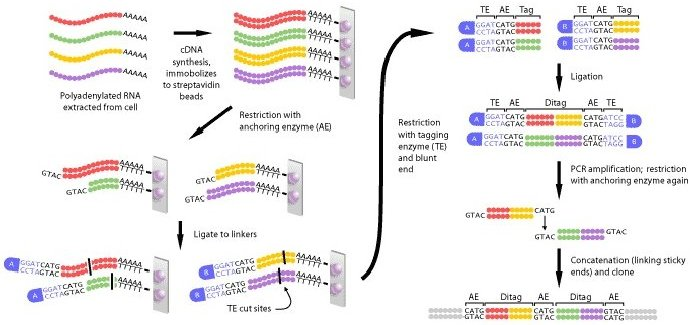
\includegraphics[width=0.8\textwidth]{c3_transcriptome/method_sage_01.jpg}
  \end{figure}
\end{frame}

\begin{frame}
  \frametitle{转录组学 | 研究方法 | MPSS}
  {\footnotesize
  \begin{block}{MPSS}
    Massive parallel signature sequencing (MPSS) is a procedure that is used to identify and quantify mRNA transcripts, resulting in data similar to serial analysis of gene expression (SAGE), although it employs a series of biochemical and sequencing steps that are substantially different.
  \end{block}
  }
  \begin{figure}
    \centering
    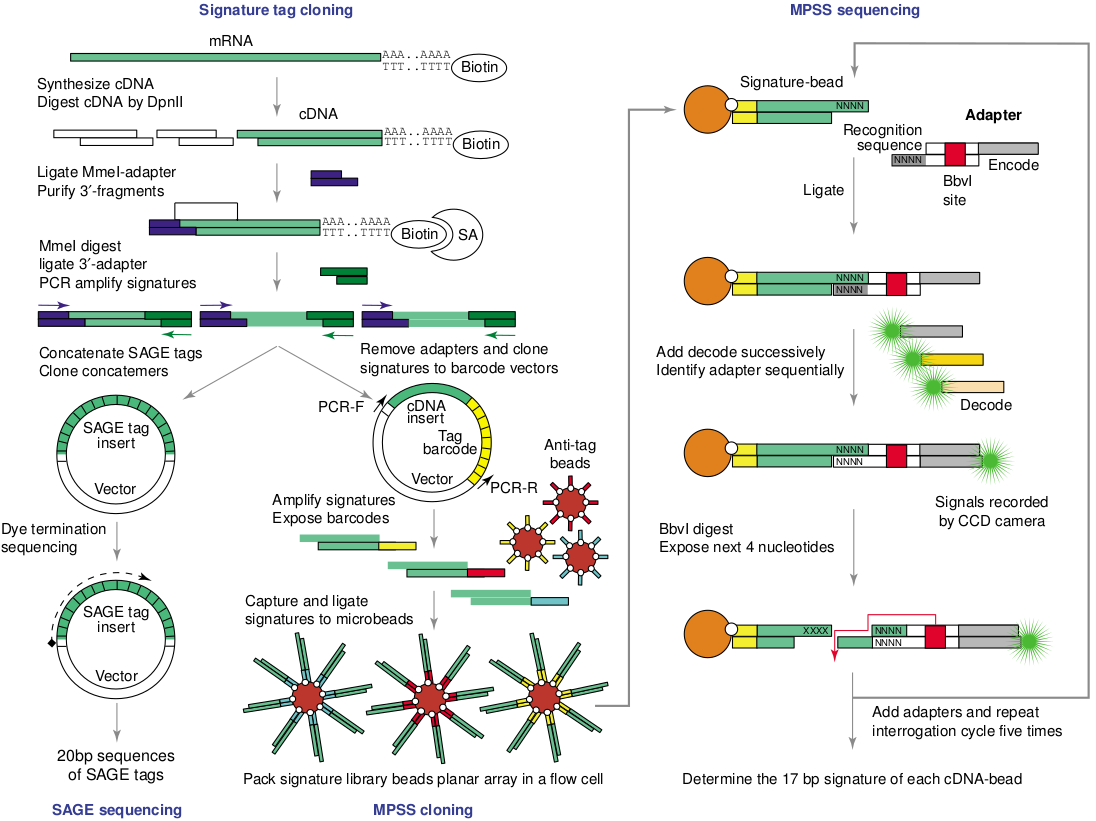
\includegraphics[width=0.6\textwidth]{c3_transcriptome/method_mpss_03.png}
  \end{figure}
\end{frame}

\begin{frame}
  \frametitle{转录组学 | 研究方法 | Microarray}
  \begin{figure}
    \centering
    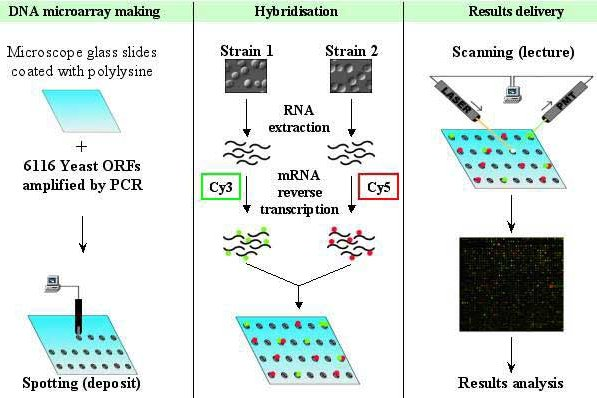
\includegraphics[width=0.9\textwidth]{c3_transcriptome/method_array_01.jpg}
  \end{figure}
\end{frame}

\begin{frame}
  \frametitle{转录组学 | 研究方法 | RNA-Seq}
  {\footnotesize
  \begin{block}{RNA-Seq}
    RNA-seq (RNA sequencing), also called whole transcriptome shotgun sequencing (WTSS), uses next-generation sequencing (NGS) to reveal the presence and quantity of RNA in a biological sample at a given moment in time.
  \end{block}
  }
  \begin{figure}
    \centering
    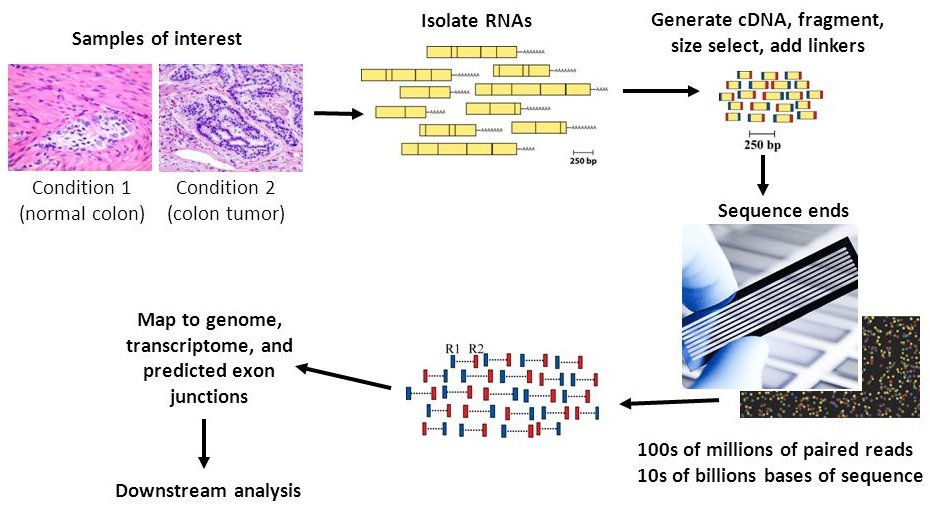
\includegraphics[width=0.8\textwidth]{c3_transcriptome/method_seq_01.jpg}
  \end{figure}
\end{frame}

\begin{frame}
  \frametitle{转录组学 | 研究方法 | \textcolor{red}{Microarray vs. RNA-Seq}}
  \begin{figure}
    \centering
    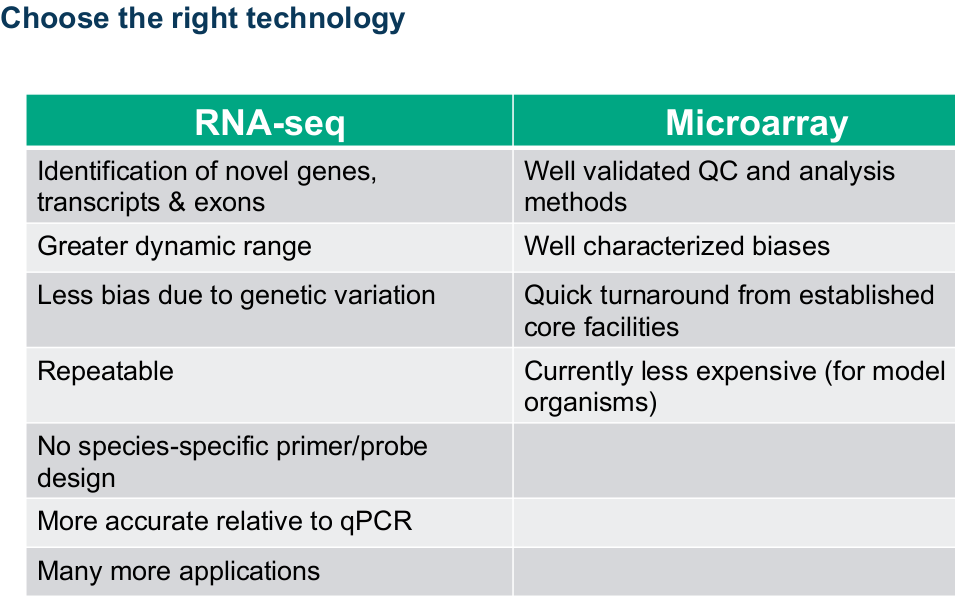
\includegraphics[width=0.9\textwidth]{c3_transcriptome/method_array_seq_01.png}
  \end{figure}
\end{frame}


